% ------------------------------------------------------------------------
% Modelo de Trabalho de Conclusão de Curso em conformidade com 
% ABNT NBR 14724:2011: Informacao e documentacao - Trabalhos academicos -
% Apresentacao
% ------------------------------------------------------------------------

\documentclass[12pt, oneside, a4paper, brazil]{abntex2}
% ---
% Pacotes básicos 
% ---
\usepackage{lmodern}			     % Usa a fonte Latin Modern			
\usepackage[T1]{fontenc}		   % Selecao de codigos de fonte.
\usepackage[utf8]{inputenc}		 % Codificacao do documento (conversão automática dos acentos)
\usepackage{lastpage}			     % Usado pela Ficha catalográfica
\usepackage{indentfirst}		   % Indenta o primeiro parágrafo de cada seção.
\usepackage{color,xcolor}			 % Controle das cores
\usepackage{graphicx}			     % Inclusão de gráficos
\usepackage{microtype} 			   % para melhorias de justificação
\usepackage[alf]{abntex2cite}	 % Citações padrão ABNT
\usepackage{lipsum}            % Pode ser removido no final
\usepackage{listingsutf8}



% Altera o nome padrão do rótulo usado no comando \autoref{}
\renewcommand{\lstlistingname}{Código}
% Altera o rótulo a ser usando no elemento pré-textual "Lista de código"
\renewcommand{\lstlistlistingname}{Lista de códigos}

% Configura a ``Lista de Códigos'' conforme as regras da ABNT (para abnTeX2)
\begingroup\makeatletter
\let\newcounter\@gobble\let\setcounter\@gobbletwo
  \globaldefs\@ne \let\c@loldepth\@ne
  \newlistof{listings}{lol}{\lstlistlistingname}
  \newlistentry{lstlisting}{lol}{0}
\endgroup

\renewcommand{\cftlstlistingaftersnum}{\hfill--\hfill}

\let\oldlstlistoflistings\lstlistoflistings
\renewcommand{\lstlistoflistings}{%
   \begingroup%
   \let\oldnumberline\numberline%
   \renewcommand{\numberline}{\lstlistingname\space\oldnumberline}%
   \oldlstlistoflistings%
   \endgroup}

\definecolor{fundo}{HTML}{DCDCDC}

\lstdefinestyle{estiloCodigos}{
    alsoother={0123456789_},
    backgroundcolor=\color{fundo},    % Cor de fundo
    basicstyle=\ABNTEXfontereduzida, 
    breakatwhitespace=false,          
    breaklines=true,                  
    captionpos=b,                     
    commentstyle=\color{green},       % cor de comentário
    deletekeywords={...},             % keywords excluídas da linguagem
    escapeinside={\%*}{*)},           % if you want to add LaTeX within your code
    extendedchars=true,               % lets you use non-ASCII characters; for 8-bits encodings only, does not work with UTF-8
    frame=single,                    % adds a frame around the code
    inputencoding=utf8,
    keepspaces=true,                 % keeps spaces in text, useful for keeping indentation of code (possibly needs columns=flexible)
    keywordstyle=\color{blue},       % keyword style
    literate={á}{{\'a}}1 {ã}{{\~a}}1 {é}{{\'e}}1 {è}{{\`{e}}}1 {ê}{{\^{e}}}1 {ë}{{\¨{e}}}1 {É}{{\'{E}}}1 {Ê}{{\^{E}}}1 {û}{{\^{u}}}1 {ú}{{\'{u}}}1 {â}{{\^{a}}}1 {à}{{\`{a}}}1 {á}{{\'{a}}}1 {ã}{{\~{a}}}1 {Á}{{\'{A}}}1 {Â}{{\^{A}}}1 {Ã}{{\~{A}}}1 {ç}{{\c{c}}}1 {Ç}{{\c{C}}}1 {õ}{{\~{o}}}1 {ó}{{\'{o}}}1 {ô}{{\^{o}}}1 {Õ}{{\~{O}}}1 {Ó}{{\'{O}}}1 {Ô}{{\^{O}}}1 {î}{{\^{i}}}1 {Î}{{\^{I}}}1 {í}{{\'{i}}}1 {Í}{{\~{Í}}}1,
    % if you want to add more keywords to the set
    morekeywords={*, :-},
    numberbychapter=false,
    numbers=left,                    % where to put the line-numbers; possible values are (none, left, right)
    numbersep=5pt,                   % how far the line-numbers are from the code
    % the style that is used for the line-numbers
    %numberstyle=\tiny\color{theframe}\sffamily, 
    numberstyle=\tiny\sffamily, 
    %rulecolor=\color{theframe},         % if not set, the frame-color may be changed on line-breaks within not-black text (e.g. comments (green here))
    showspaces=false,                % show spaces everywhere adding particular underscores; it overrides 'showstringspaces'
    showstringspaces=false,          % underline spaces within strings only
    showtabs=false,                  % show tabs within strings adding particular underscores
    stepnumber=1,                    % the step between two line-numbers. If it's 1, each line will be numbered
    %stringstyle=\color{mymauve}\itshape,     % string literal style
    stringstyle=\ttfamily,     % string literal style
    tabsize=2,                       % sets default tabsize to 2 spaces
    title=\lstname,                  % show the filename of files included with \lstinputlisting; also try caption instead of title
    framexleftmargin=10pt,
    framexleftmargin=15pt
}
\lstset{escapechar=@,style=estiloCodigos}


\titulo{Modelo de Trabalho de Conclusão \\ do IFC -- Araquari usando \abnTeX}
\autor{Nome do Aluno}
\local{Araquari -- SC}
\data{Julho de 2016}
\orientador{Prof. Dr. Fernando José Braz}
\coorientador{Prof. Dr. Nome do Coorientador}
\titulo{Modelo de Trabalho de Conclusão \\ do IFC -- Araquari usando \abnTeX}
\autor{Cláudio César Gonçalves de Faria Filho}
\local{Araquari -- SC}
\data{Julho de 2016}
\orientador{Prof. Dr. Fernando José Braz}
\coorientador{Prof. Dr. Nome do Coorientador}
% Informações de dados para CAPA e FOLHA DE ROSTO
\instituicao{%
  Instituto Federal Catarinense -- IFC
  \par
  Câmpus Araquari
  \par
  Bacharelado em Sistemas de Informação}
\tipotrabalho{Monografia (Graduação)}
% O preambulo deve conter o tipo do trabalho, o objetivo, 
% o nome da instituição e a área de concentração 
\preambulo{Trabalho de conclusão de curso apresentado como requisito parcial para a obtenção do grau de bacharel em Sistemas de Informação do Instituto Federal Catarinense.}


% Configurações de aparência do PDF final
% informações do PDF
\makeatletter
\hypersetup{
   	%pagebackref=true,
		pdftitle={\@title}, 
		pdfauthor={\@author},
   	pdfsubject={\imprimirpreambulo},
    pdfcreator={LaTeX with abnTeX2},
		pdfkeywords={abnt}{latex}{abntex}{abntex2}{trabalho acadêmico}, 
		colorlinks=true,       		% false: boxed links; true: colored links
   	linkcolor=blue,          	% color of internal links
   	citecolor=blue,        		% color of links to bibliography
   	filecolor=magenta,     		% color of file links
		urlcolor=blue,
		bookmarksdepth=4
}
\makeatother

% Espaçamentos entre linhas e parágrafos 

\setlength{\parindent}{1.3cm}			% O tamanho do parágrafo é dado por:
\setlength{\parskip}{0.2cm}  			% Controle do espaçamento entre um parágrafo e outro:


% Início do documento
\begin{document}
%\selectlanguage{english}
\selectlanguage{brazil} 				% Seleciona o idioma do documento (conforme pacotes do babel)
\frenchspacing 							    % Retira espaço extra obsoleto entre as frases.

% ELEMENTOS PRÉ-TEXTUAIS
\imprimircapa							% Capa
\imprimirfolhaderosto*		% Folha de rosto
								          % (o * indica que haverá a ficha bibliográfica)

% Inserir a ficha bibliografica

% Isto é um exemplo de Ficha Catalográfica, ou ``Dados internacionais de 
% catalogação-na-publicação''. Utilizar este modelo como referência. 
% Porém, provavelmente a biblioteca fornecerá um PDF com a ficha catalográfica 
% definitiva após a defesa do trabalho. Quando estiver com o documento, salve-o como PDF 
% no diretório do seu projeto e substitua todo o conteúdo de implementação deste arquivo 
% pelo comando abaixo:
%
% \begin{fichacatalografica}
%     \includepdf{fig_ficha_catalografica.pdf}
% \end{fichacatalografica}

\begin{fichacatalografica}
	\sffamily
	\vspace*{\fill}					% Posição vertical
	\begin{center}					% Minipage Centralizado
	\fbox{\begin{minipage}[c][8cm]{13.5cm}		% Largura
	\small
	\imprimirautor
	%Sobrenome, Nome do autor
	
	\hspace{0.5cm} \imprimirtitulo  / \imprimirautor. --
	\imprimirlocal, \imprimirdata-
	
	\hspace{0.5cm} \pageref{LastPage} p. : il. (algumas color.) ; 30 cm.\\
	
	\hspace{0.5cm} \imprimirorientadorRotulo~\imprimirorientador\\
	
	\hspace{0.5cm}
	\parbox[t]{\textwidth}{\imprimirtipotrabalho~--~\imprimirinstituicao,
	\imprimirdata.}\\
	
	\hspace{0.5cm}
		1. Palavra-chave1.
		2. Palavra-chave2.
		2. Palavra-chave3.
		I. Orientador.
		II. Instituto Federal Catarinense.
		III. Câmpus Araquari.
		IV. Título 			
	\end{minipage}}
	\end{center}
\end{fichacatalografica}
% ---



% Inserir folha de aprovação

% Exemplo de Folha de aprovação, elemento obrigatório da NBR 14724/2011 (seção 4.2.1.3). 
% Utilizar este modelo até a aprovação do trabalho. Após isso, substitua todo o conteúdo 
% deste arquivo por uma imagem da página assinada pela banca com o comando abaixo:
%
% \includepdf{folhadeaprovacao_final.pdf}
%
\begin{folhadeaprovacao}

  \begin{center}
    {\ABNTEXchapterfont\large\imprimirautor}

    \vspace*{\fill}\vspace*{\fill}
    \begin{center}
      \ABNTEXchapterfont\bfseries\Large\imprimirtitulo
    \end{center}
    \vspace*{\fill}
    
    \hspace{.45\textwidth}
    \begin{minipage}{.5\textwidth}
        \imprimirpreambulo
    \end{minipage}%
    \vspace*{\fill}
   \end{center}
        
   Trabalho aprovado. \imprimirlocal, 24 de novembro de 2016:

   \assinatura{\textbf{\imprimirorientador} \\ Orientador} 
   \assinatura{\textbf{Professor} \\ Convidado 1}
   \assinatura{\textbf{Professor} \\ Convidado 2}
   %\assinatura{\textbf{Professor} \\ Convidado 3}
   %\assinatura{\textbf{Professor} \\ Convidado 4}
      
   \begin{center}
    \vspace*{0.5cm}
    {\large\imprimirlocal}
    \par
    {\large\imprimirdata}
    \vspace*{1cm}
  \end{center}
  
\end{folhadeaprovacao}
% ---

% Dedicatória
\begin{dedicatoria}
   \vspace*{\fill}
   \centering
   \noindent
   \textit{ Dedicatória do trabalho de conclusão que deve \\
   ser algo breve e conciso.} \vspace*{\fill}
\end{dedicatoria}


% Agradecimentos
\begin{agradecimentos}
Página com os agradecimentos do autor à pessoas importantes para a realização do trabalho.
\end{agradecimentos}

% Epígrafe
\begin{epigrafe}
    \vspace*{\fill}
	\begin{flushright}
		\textit{``Colocar alguma frase importante que, \\
		tenha motivado o autor no decorrer do desenvolvimento \\
		do trabalho.'' \\
		(Referência de local da frase)}
	\end{flushright}
\end{epigrafe}

% RESUMOS
% resumo em português
\setlength{\absparsep}{18pt} % ajusta o espaçamento dos parágrafos do resumo
\begin{resumo}
 Segundo a \citeonline[3.1-3.2]{NBR6028:2003}, o resumo deve ressaltar o
 objetivo, o método, os resultados e as conclusões do documento. A ordem e a extensão
 destes itens dependem do tipo de resumo (informativo ou indicativo) e do
 tratamento que cada item recebe no documento original. O resumo deve ser
 precedido da referência do documento, com exceção do resumo inserido no
 próprio documento. (\ldots) As palavras-chave devem figurar logo abaixo do
 resumo, antecedidas da expressão Palavras-chave:, separadas entre si por
 ponto e finalizadas também por ponto.

 \textbf{Palavras-chave}: latex. abntex. editoração de texto.
\end{resumo}

% resumo em inglês
\begin{resumo}[Abstract]
 \begin{otherlanguage*}{english}
   This is the english abstract.

   \vspace{\onelineskip}
 
   \noindent 
   \textbf{Keywords}: latex. abntex. text editoration.
 \end{otherlanguage*}
\end{resumo}


% ---
% inserir lista de ilustrações
% ---
\pdfbookmark[0]{\listfigurename}{lof}
\listoffigures*
\cleardoublepage
% ---

% ---
% inserir lista de tabelas
% ---
\pdfbookmark[0]{\listtablename}{lot}
\listoftables*
\cleardoublepage
% ---
% inserir lista de codigos
% ---
\pdfbookmark[0]{\lstlistlistingname}{lol}
\begin{KeepFromToc}
\lstlistoflistings
\end{KeepFromToc}
\cleardoublepage
% ---

% ---
% inserir lista de abreviaturas e siglas
% ---
\begin{siglas}
  \item[ABNT] Associação Brasileira de Normas Técnicas
  \item[abnTeX] ABsurdas Normas para TeX
\end{siglas}
% ---

% ---
% inserir lista de símbolos
% ---
\begin{simbolos}
  \item[$ \Gamma $] Letra grega Gama
  \item[$ \Lambda $] Lambda
  \item[$ \zeta $] Letra grega minúscula zeta
  \item[$ \in $] Pertence
\end{simbolos}
% ---

% ---
% inserir o sumario
% ---
\pdfbookmark[0]{\contentsname}{toc}
\tableofcontents*
\cleardoublepage
% ---

% ----------------------------------------------------------
% ELEMENTOS TEXTUAIS
% ----------------------------------------------------------
\textual

% ---
% Inclusão de capítulo de Introdução ao trabalho
% ---
% ----------------------------------------------------------
% Introdução (exemplo de capítulo sem numeração, mas presente no Sumário)
% ----------------------------------------------------------
\chapter[Introdução]{Introdução}
%\addcontentsline{toc}{chapter}{Introdução}
% ----------------------------------------------------------

Com a crescente demanda de soluções tecnológicas para resolução de problemas cotidianos governamentais, o conceito de cidades inteligentes se torna cada vez mais necessário na gestão de políticas públicas. O crescimento da produção de dados de geolocalização, gerado pela crescente aderência populacional ao uso de \textit{smartphones}, criou um ambiente propício para o desenvolvimento de aplicativos utilizando essa tecnologia.

Este trabalho propõe o desenvolvimento de um algoritmo para identificação do agrupamento de trajetórias com comportamento similares. As trajetórias representam a movimentação de usuários de transporte público quando desembarcados.
% ---
% Inclusão de outros capitulos
% ---
\chapter{Lorem ipsum dolor sit amet}

É importante apresentar, ao início de cada capítulo, uma breve introdução sobre o mesmo. Essa introdução, não deve conter mais do que 2 parágrafos. Uma sugestão, é relembrar de forma sucinta o que foi apresentado no capítulo anterior, e relacionar com o conteúdo deste capítulo.

Também é aconselhável, que cada capítulo possua uma sessão de conclusão. A importância desta é discutida adiante. Esta recomendações não são uma regra do IFC, mas têm sido bastante utilizadas no BSI. 

\section{Figuras e legendas}\label{sec:figs}

Essa sessão apresenta como utilizar figuras e tabelas ao longo do TCC. Também é apresentado o uso das legendas para esses dois tipos de recursos. 

Temos dois exemplos, a figura~\ref{fig:exemploFig1} e a figura~\ref{fig:exemploFig2}.

\begin{figure}[htbp]
\centering
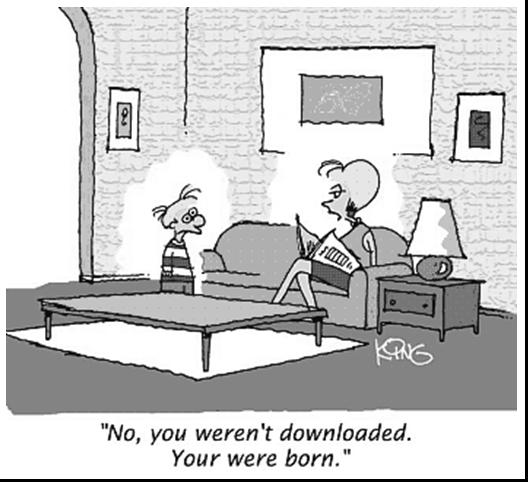
\includegraphics[width=.5\textwidth]{figuras/fig1.jpg}
\caption{Uma figura típica}
\label{fig:exemploFig1}
\end{figure}

\begin{figure}[htbp]
\centering
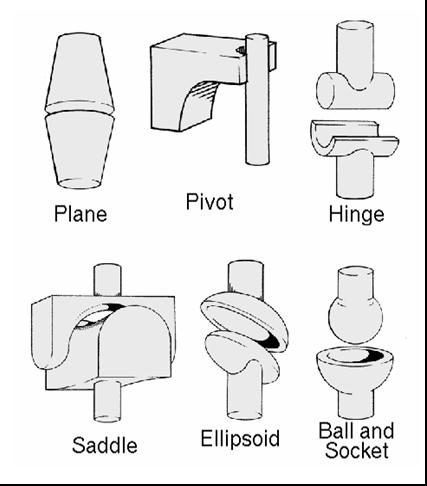
\includegraphics[width=.3\textwidth]{figuras/fig2.jpg}
\caption{Essa figura é um exemplo de figura contendo uma legenda utilizando mais do que uma única linha.}
\label{fig:exemploFig2}
\end{figure}

A figura~\ref{fig:exemplo_png} que é um exemplo de figura no formato PNG. Além desse formato, também pode-se utilizar figuras no formato JPG e GIF. Figuras no formato EPS também podem ser utilizadas, porém a geração do PDF final não pode ser feita utilizando diretamente o comando \texttt{pdflatex}.

\begin{figure}[htbp]
\centering

\includegraphics[width=.5\textwidth]{figuras/latex-logo.png}
\caption{Essa figura é um exemplo de figura no formato PNG.}
\label{fig:exemplo_png}
\end{figure}

Podemos utilizar tabelas também (tabela~\ref{tab:exTabela}). Nesse caso tente evitar o uso de fundos com cores ou sombras, e evite linhas de grade grossas, duplas ou desnecessárias. A legenda da tabela deve ser colocada sempre antes dela, no topo.

\begin{table}[htbp]
\centering
\caption{Um exemplo de tabela}
\label{tab:exTabela}
\begin{tabular}{l|c|r} \hline
Cabeçalho Esquerda & Cabeçalho Centro & Cabeçalho Direita \\ 
\hline \hline
Linha 1 Coluna 1   & Linha 1 Coluna 2 & Linha 1 Coluna 3  \\
Linha 2            & Coluna do meio   & Coluna 3          \\
Coluna 1           & Linha 3          & Última célula     \\
\hline
\end{tabular}
\end{table}

\section{Códigos-fontes de linguagens de programação}

Uma linguagem de programação é um método padronizado para expressar instruções para um computador. É um conjunto de regras sintáticas e semânticas usadas para definir um programa de computador. Uma linguagem permite que um programador especifique precisamente sobre quais dados um computador vai atuar, como estes dados serão armazenados ou transmitidos e quais ações devem ser tomadas sob várias circunstâncias.

Depois que inventaram o computador , perceberam que ele não servia prá nada. Durante milhares de anos o computador ficou relegado a segundo plano e apenas calculadoras eram usadas! Mas um tecelão francês chamado Jacquard criou o primeiro programa para suas máquinas de tecer. Com inveja, Blaise Pascal, inventou a linguagem Pascal para jovens com retardamento mental. Naquela época os computadores ainda eram muito rudimentares e não foi possível utilizar de forma satisfatória todos os recursos das Linguagens de Programação. Muito tempo depois Charles Babbage criou a máquina Diferencial prá fazer subtrações e a máquina Somatorial para fazer somas. Como dava um trabalho muito duro construir máquinas para cada uma das operações, ele pediu à sua assistente Lady Ada Lovelace prá resolver o problema. Ada então criou a Linguagem de Programação Ada, muito utilizada na Guerra do Golfo pelos Militares Americanos.

\subsection{Python}

Python é uma linguagem de programação de alto-nível interpretada, interativa, orientada a objetos, de tipagem dinâmica e forte. A linguagem foi projetada com a filosofia de enfatizar a importância do esforço do programador sobre o esforço computacional. Prioriza a legibilidade do código sobre a velocidade ou expresividade. Combina uma sintaxe concisa e clara com os recursos poderosos de sua biblioteca padrão e por módulos e frameworks desenvolvidos por terceiros. O código \ref{mediapy} é um exemplo de código-fonte em Python.

%\begin{figure}[htbp] 
\lstinputlisting[language=python,caption={Cálculo da média entre dois números escrito na linguagem Python},label=mediapy]{codigos/media.py}
%\centering
%\caption{Cálculo da média entre dois números escrito na linguagem Python}
%\label{fig:mediapy}\end{figure}

Python é a principal sucessora de Logo, porém é também uma calculadora de linha de comando, orientada à identação. Costuma ser o destino preferencial dos programadores Ruby, quando estes finalmente se dão conta que estão usando um ``Perl 2.0''. 

\subsection{C++}

O C++ é uma linguagem de programação de alto nível com facilidades para o uso em baixo nível, multiparadigma e de uso geral. Desde os anos 1990 é uma das linguagens comerciais mais populares, sendo bastante usada também na academia por seu grande desempenho e base de utilizadores.  O código \ref{mediacpp} é um exemplo de código-fonte em C++.

%\begin{figure}[htbp]
\lstinputlisting[language=C++, caption={Cálculo da média entre dois números escrito na linguagem C++}, label=mediacpp]{codigos/media.cpp}
%\centering
%\caption{Cálculo da média entre dois números escrito na linguagem C++}
%\label{fig:mediacpp}
%\end{figure}

C++ é uma linguagem de programação, muitas vezes é referida como Cpp , criada por Steve Ballmer com o propósito de deixar programador loucos, em um plano para eliminar a concorrência da Microsoft (que usa a programação orientada a gambiarras em seus programas).

Suas principais características são o paradigma orientado à desorientação e falta de sentido em geral, a incoerência de sintaxe, e ser melhor do que Java. A linguagem incorpora todas as vantagens da linguagem C, isto é, nenhuma, e todos os benefícios da orientação a objetos, isto é, poder fazer uma classe Quadrado que herda da classe Retângulo, com um incrivel custo em performance por isso. 

\subsection{Java}

Java é uma linguagem de programação orientada a objeto desenvolvida na década de 90 pelo programador James Gosling, na empresa Sun Microsystems. Diferentemente das linguagens convencionais, que são compiladas para código nativo, a linguagem Java é compilada para um ``bytecode'' que é executado por uma máquina virtual. A linguagem de programação Java é a linguagem convencional da Plataforma Java, mas não sua única linguagem.  O código \ref{mediajava} é um exemplo de código-fonte em Java.

%\begin{figure}[htbp]
\lstinputlisting[language=java, caption={Cálculo da média entre dois números escrito na linguagem Java}, label=mediajava]{codigos/media.java}
%\caption{Cálculo da média entre dois números escrito na linguagem Java}
%\label{fig:mediajava}
%\end{figure}

A Linguagem Java é famosa por ser muito eficiente. A maioria dos programas mais complexos é escrita em Java, como o Adobe Photoshop ou o Microsoft Windows ME, podendo funcionar com apenas 640 bytes de RAM, e atingir velocidades instantâneas. Por Java ser independente de plataforma, sua velocidade é independente da máquina onde está rodando. Por padrão, Java 1.2 pode calcular um loop infinito em menos de 1.2 minutos, daí vem esse número na linguagem. A palavra ``Java'' vem de um dialeto da Indonésia que quer dizer ``Espetáculo do crescimento'', o que explica programas com poucos KBytes no disco possuírem dezenas de MBytes na memória principal.

\subsection{Listas numeradas e de itens}

Se quisermos uma lista numerada, devemos fazer assim:

\begin{enumerate}
\item este é o primeiro item;
\item este é o segundo item;
\item e este é o terceiro e último item.
\end{enumerate}

Por outro lado, uma lista de itens é feita desse modo:

\begin{itemize}
\item este é o primeiro item;
\item este é o segundo item;
\item e este é o terceiro e último item.
\end{itemize}

\section{Referências}

Referências bibliográficas precisam ser não ambíguas e uniformes. Recomendamosdar os nomes dos autores entre espaços, por exemplo \cite{knuth:84},
\cite{boulic:91}, e \cite{smith:99}. Em caso de dúvidas, consulte o manual de metodologia para desenvolvimento do TCC, disponível na página do IFC ou na página do BSI.

Citações longas com mais de três linhas devem seguir ao seguinte formato:

\begin{citacao}
O IPSEC foi concebido como uma extensão de terceira camada ao TCP/IP, ou seja estende o próprio protocolo IP. Na verdade, para o IPv6; depois o IPSEC também foi portado para o IPv4.
A idéia original do IPSEC é permitir a comunicação segura e *transparente* entre quaisquer dois nós da Internet, desde que os dois implementem IPSEC. Se os dois têm IPSEC, automaticamente há troca de chaves e criptografia. Esse modo de funcionamento do IPSEC denomina-se ``modo transporte''~\cite{epx}. 
\end{citacao}

% ---
\section{Aliquam vestibulum fringilla lorem}
% ---

\lipsum[1]

\lipsum[2-3]

% ---
% primeiro capitulo de Resultados
% ---
\chapter{Lectus lobortis condimentum}
% ---

% ---
\section{Vestibulum ante ipsum primis in faucibus orci luctus et ultrices
posuere cubilia Curae}
% ---

\lipsum[21-22]

% ---
% segundo capitulo de Resultados
% ---
\chapter{Nam sed tellus sit amet lectus urna ullamcorper tristique interdum
elementum}
% ---

% ---
\section{Pellentesque sit amet pede ac sem eleifend consectetuer}
% ---

\lipsum[24]


% ----------------------------------------------------------
% Finaliza a parte no bookmark do PDF
% para que se inicie o bookmark na raiz
% e adiciona espaço de parte no Sumário
% ----------------------------------------------------------
\phantompart

% ---
% Conclusão
% ---
\chapter{Conclusão}
% ---

\lipsum[31-33]


% ----------------------------------------------------------
% ELEMENTOS PÓS-TEXTUAIS
% ----------------------------------------------------------
\postextual
% ----------------------------------------------------------

% ----------------------------------------------------------
% Referências bibliográficas
% ----------------------------------------------------------
\bibliography{referencias}

% ----------------------------------------------------------
% Glossário
% ----------------------------------------------------------
%
% Consulte o manual da classe abntex2 para orientações sobre o glossário.
%
%\glossary

% ----------------------------------------------------------
% Apêndices
% ----------------------------------------------------------

% ---
% Inicia os apêndices
% ---
\begin{apendicesenv}

% Imprime uma página indicando o início dos apêndices
\partapendices

% ----------------------------------------------------------
\chapter{Quisque libero justo}
% ----------------------------------------------------------

\lipsum[50]

% ----------------------------------------------------------
\chapter{Nullam elementum urna vel imperdiet sodales elit ipsum pharetra ligula
ac pretium ante justo a nulla curabitur tristique arcu eu metus}
% ----------------------------------------------------------
\lipsum[55-57]

\end{apendicesenv}
% ---


% ----------------------------------------------------------
% Anexos
% ----------------------------------------------------------

% ---
% Inicia os anexos
% ---
\begin{anexosenv}

% Imprime uma página indicando o início dos anexos
\partanexos

% ---
\chapter{Morbi ultrices rutrum lorem.}
% ---
\lipsum[30]

% ---
\chapter{Cras non urna sed feugiat cum sociis natoque penatibus et magnis dis
parturient montes nascetur ridiculus mus}
% ---

\lipsum[31]

% ---
\chapter{Fusce facilisis lacinia dui}
% ---

\lipsum[32]

\end{anexosenv}

%---------------------------------------------------------------------
% INDICE REMISSIVO
%---------------------------------------------------------------------
\phantompart
\printindex
%---------------------------------------------------------------------

\end{document}
